%=====================================================================
\section{Training}
\label{sec:training}

\subsection{Training instances}
\label{sec:generator}

\code{rl2\_generator.py} makes a new random instance for every training episode, with the rules that built the EV-Solomon dataset (\code{make\_ev\_solomon.py}). From the CSV dataset it takes one \emph{template} per (file size, Solomon class): planning period $T$, depot, city area, number of stations, guns and power, costs and fleet. For each instance it then draws new customers:
\begin{itemize}
  \item \textbf{positions}: class R uniform in the city area; class C in 5--12 Gaussian clusters listed cluster by cluster (as in Solomon, so the first $n$ EVs are concentrated); class RC half clustered, half uniform;
  \item \textbf{stations}: $k$-means of all customer positions (the dataset's rule);
  \item \textbf{energy}: Solomon demand $1\ldots50$ mapped linearly onto $[10,40]$ kWh;
  \item \textbf{range}: uniform, and 15\,\% of the EVs ``stranded'' with 20--80\,\% of the distance to their nearest station;
  \item \textbf{request times}: a share (15--30\,\%) at time 0, the rest $T\cdot u\cdot\mathrm{Beta}(a,b)$ with $u\in[0.83,0.92]$, $a=1$, $b=2.5$, rounded to minutes (fitted to the dataset's request times);
  \item \textbf{income}: $\theta\sim\mathrm{Beta}$ with the parameters of \code{f3\_params.json};
  \item \textbf{period}: the class's $T$ times a random factor in $[0.85,1.15]$.
\end{itemize}
As in the dataset, an instance is the first $n$ EVs of a full random file of 100. Each instance of a batch gets a random class and a random map symmetry.

\subsection{Phase 1: imitation warm-up}

For the first 500 batches (10 epochs) the greedy cost rule plays every episode and the policy learns to reproduce its actions:
\[
\mathcal L_{\text{IL}}(\phi)=-\frac1n\,\frac1B\sum_{b=1}^{B}\sum_{t}\log p_\phi\big(a^{\text{rule}}_{b,t}\mid s_{b,t}\big).
\]
A warm-up batch is about 8 times cheaper than a REINFORCE batch, because each instance is played once instead of $S=8$ times.

\begin{whybox}[title=Why a warm-up]
From random weights the untrained policy costs 1.4--1.8 times the greedy rule on the validation instances (RL1 server log: 1.43 at epoch 0). On the laptop, pure REINFORCE needed many batches to approach the rule (1.18 after 77 batches), while imitation reached about 1.00 after a few hundred cheap batches; on the server the first warm-up epoch already gave 1.014. REINFORCE then starts from a sensible policy and only has to learn where to deviate from the rule.
\end{whybox}

\subsection{Phase 2: REINFORCE with a shared baseline}

Each batch has $B$ random instances with the same $n$ (64 in RL2, 32 in RL1). The encoder runs once per instance; every instance is then rolled out $S=8$ times by sampling. For rollout $j$ of instance $b$ let $\tilde c_{bj}$ be its penalised cost (Assumption~\ref{as:penalty}). The baseline and the advantage are
\[
\bar c_b=\frac1S\sum_{j=1}^{S}\tilde c_{bj},\qquad A_{bj}=\frac{\tilde c_{bj}-\bar c_b}{\bar c_b},
\]
and the loss whose gradient is the REINFORCE estimator is
\[
\mathcal L_{\text{RL}}(\phi)=\frac{1}{BS}\sum_{b,j}A_{bj}\,\log p_\phi(\pi_{bj}\mid x_b),\qquad
\nabla_\phi\mathcal L_{\text{RL}}\approx\nabla_\phi\,\E\Big[\frac{\tilde c}{\bar c}\Big].
\]
Rollouts cheaper than their instance's mean get a negative advantage, and the gradient step makes their actions more likely.

\begin{whybox}[title=Why this baseline and this normalisation]
\begin{itemize}
  \item The mean of the other rollouts of the same instance is a good estimate of ``what this policy usually achieves on this instance'', without a critic network to train and without the extra greedy rollout of a frozen policy copy that Kool et al.\ use.
  \item The mean includes the rollout itself; this multiplies the expected gradient by $(S-1)/S$ but does not change its direction.
  \item Dividing by $\bar c_b$ makes the advantage a relative cost. $Z$ differs by orders of magnitude between classes and sizes; without the division, the largest instances would dominate every batch.
\end{itemize}
\end{whybox}

\textbf{Optimiser.} Adam, gradient norm clipped at 1.0. Learning rate $10^{-4}$ during the warm-up and $2\times10^{-5}$ for REINFORCE, both multiplied by $0.9998^{\text{epoch}}$.

\subsection{Validation, stopping and saving}

After every epoch (50 batches) the policy's \emph{greedy} rollout is compared with the greedy cost rule on fixed validation instances (seed 777):
\[
\text{ratio}=\text{mean over validation instances of }\ \frac{\tilde c(\text{policy, greedy})}{\tilde c(\text{greedy rule})}.
\]
The network of the epoch with the lowest ratio is saved as \code{model\_best.pt}; the solver uses this one. Training stops at the first of:
\begin{itemize}
  \item \code{max\_epochs} $=500$ epochs in total;
  \item early stop: 10 REINFORCE epochs in a row without a better ratio, counted only after the first \code{min\_epochs} $=200$ epochs (so the earliest stop is at epoch 210);
  \item the time cap (8 hours).
\end{itemize}
Every run starts at epoch 1 with new weights; the files of the previous run are moved to \code{model/previous\_runs/<date-time>/}. A batch that fails is logged and skipped (training stops only after 20 failures in a row), and Ctrl-C saves the model first.

\subsection{What RL2 changes in training, and why}

\begin{center}\small
\begin{tabular}{@{}lll@{}}
\toprule
\textbf{Setting} & \textbf{RL1} & \textbf{RL2} \\
\midrule
instances per batch & 32 & 64 \\
rollouts per batch ($B\times S$) & 256 & 512 \\
distribution of $n$ in a batch & uniform on $[10,100]$ & $P(n)\propto n$ on $[10,100]$ \\
mean training $n$ & 55.0 & 67.5 \\
share of batches with $n\ge60$ & 45\,\% & 66\,\% \\
validation instances & $3\times24=72$ ($n=20,50,100$) & $4\times50=200$ ($n=20,50,80,100$) \\
\bottomrule
\end{tabular}
\end{center}

\begin{figure}[h]
\centering
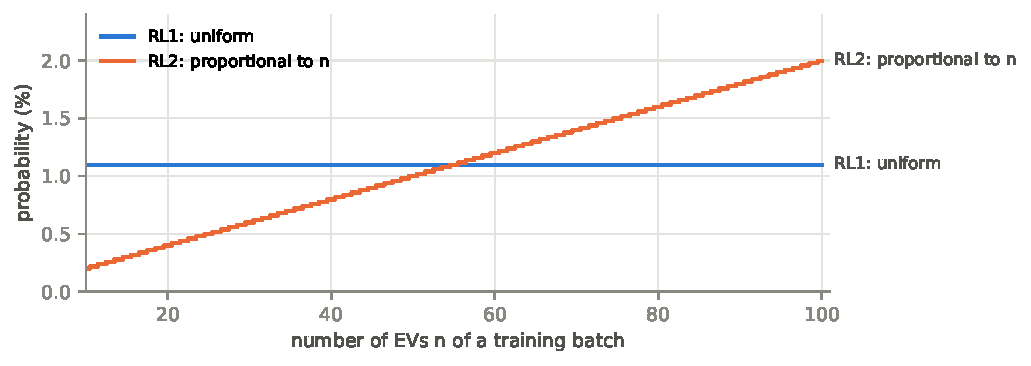
\includegraphics[width=0.85\textwidth]{figures/rl2_n_weighting.pdf}
\caption{Probability of each $n$ for a training batch. RL2 draws $n$ with probability proportional to $n$, so large instances, where RL1 lost most against the MILP, are trained more often.}
\label{fig:nweight}
\end{figure}

\begin{enumerate}
  \item \textbf{Batch 64.} The variance of the gradient estimate falls roughly as $1/(BS)$. RL1's validation ratio moved by $\pm0.003$ from epoch to epoch after epoch 150 (Figure~\ref{fig:train}), so a less noisy gradient is the first thing to try. An epoch takes about twice as long.
  \item \textbf{$P(n)\propto n$.} RL1's gap to the MILP rises from 0.5\,\% at $n=10$ to 1.5--1.7\,\% at $n=60$--$90$ (Figure~\ref{fig:gapn}). Weighting by $n$ trains these sizes more often while still covering small $n$. A batch with large $n$ also has more decisions, so more of the learning signal comes from the hard part of the plan.
  \item \textbf{200 validation instances.} The best epoch is chosen as the minimum of a noisy curve, which favours an epoch that was lucky on the validation set. With 200 instances instead of 72 the standard error of the ratio falls by a factor of about $\sqrt{200/72}\approx1.7$, and $n=80$ is now checked directly.
\end{enumerate}
